\documentclass[12pt]{article}
\usepackage[english]{babel}
\usepackage{float}
\usepackage[margin=1in]{geometry}
\usepackage{graphicx}
%\usepackage[toc,page]{appendix}
\graphicspath{ {./doc/img/} }
\newcommand{\rpm}{\raisebox{.2ex}{$\scriptstyle\pm$}} 
\usepackage{listings}
\usepackage{xcolor}
\usepackage{indentfirst}
\usepackage[final]{pdfpages}


\begin{document}

\title{Joe Phaneuf \\ Computer Vision 16-720 Spring 2018 \\ Feb. 03, 2018 }
\date{}
\author{}
\maketitle

\newpage


\stepcounter{section}
%%%%%%%%%%%%%%%%%%%%%%%%%%%%%%%%%%%%%%%%%%%%%%%%%%%%%%%%%%%%%%%%%%%%%%%%%%%%%%%%
%%%%%%%%%%%%%%%%%%%%%%%%%%%%%%%%%%%%%%%%%%%%%%%%%%%%%%%%%%%%%%%%%%%%%%%%%%%%%%%%
\section{Q1}
\subsection{Q1.1}

The filter bank contains four types of filters at different scales. The first two filters (gaussian and log) will respond to circular elements, the former containing peaks and the latter containing valleys.
The next two filter types are derivitive filters, which will respond to vertical and horizontal edges respectively.
Figure \ref{fig:test_image} shows a test image for the filters, Figure shows \ref{fig:filters} the filters themselves, while Figure \ref{fig:filter_responses} shows the filtered images.

\begin{figure}[H]
\centering

\includegraphics[page=1,width=0.4\textwidth]{test}
\caption{Test image}    
\label{fig:test_image}
\end{figure}   

\begin{figure}[H]
\centering
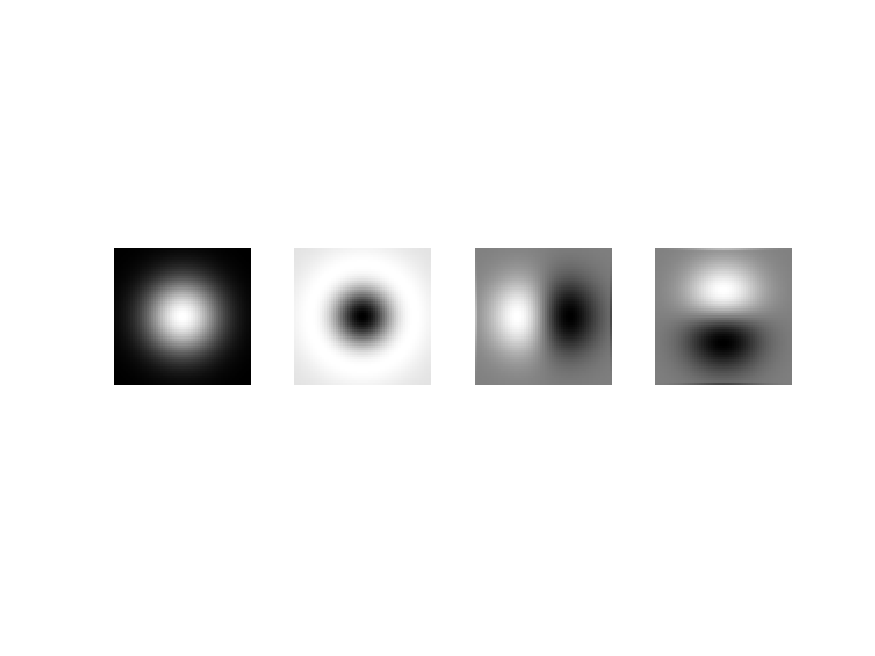
\includegraphics[page=1,width=0.75\textwidth]{q1_filters}
\caption{Filters}    
\label{fig:filters}
\end{figure}   

\begin{figure}[H]
\centering
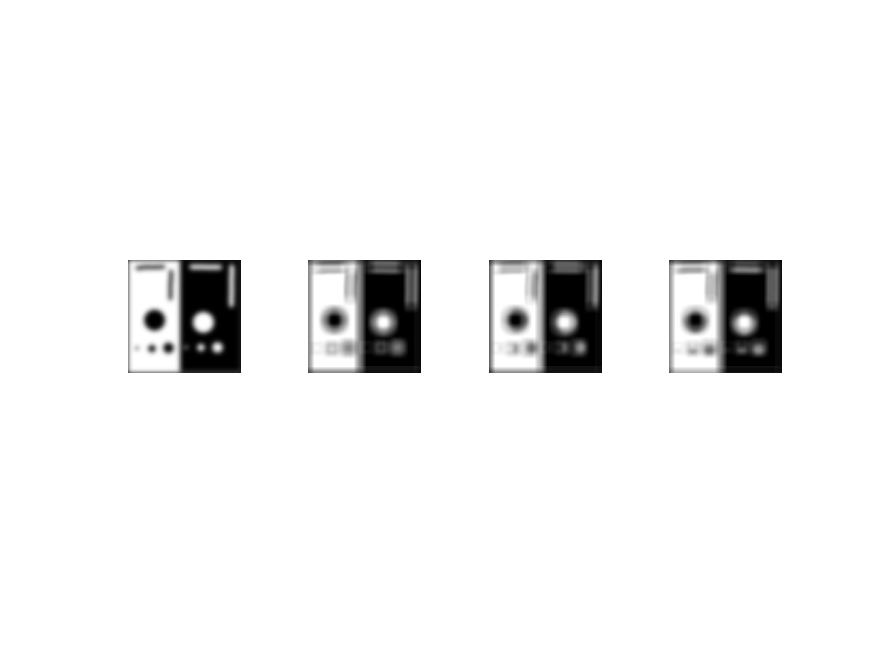
\includegraphics[page=1,width=0.75\textwidth]{q1_responses}
\caption{Filter responses}    
\label{fig:filter_responses}
\end{figure}   

%%%%%%%%%%%%%%%%%%%%%%%%%%%%%%%%%%%%%%%%%%%%%%%%%%%%%%%%%%%%%%%%%%%%%%%%%%%%%%%%
%%%%%%%%%%%%%%%%%%%%%%%%%%%%%%%%%%%%%%%%%%%%%%%%%%%%%%%%%%%%%%%%%%%%%%%%%%%%%%%%
\newpage
\subsection{Q1.2}
The extractFilterResponses function convertes an input image to the CIE LAB color space, and subsequently applies the filter bank described above to each channel (L A B).
The CIE LAB color space is chosen for this application as the image intensity is stored in a separate channel (L) from color information (A B). In RGB colorspace (default for most input images), image intensity is a combination of all channels, and image processing techniques are therefore highly sensitive to the lighting conditions in which the image was captured. The CIE LAB color space color channels will be more similar for images of the same object in different lighting conditions. Figure \ref{fig:extract_filter_responses} shows a sample image along with one feature filter applied to the L, A, and B channels.

\begin{figure}[H]
\centering
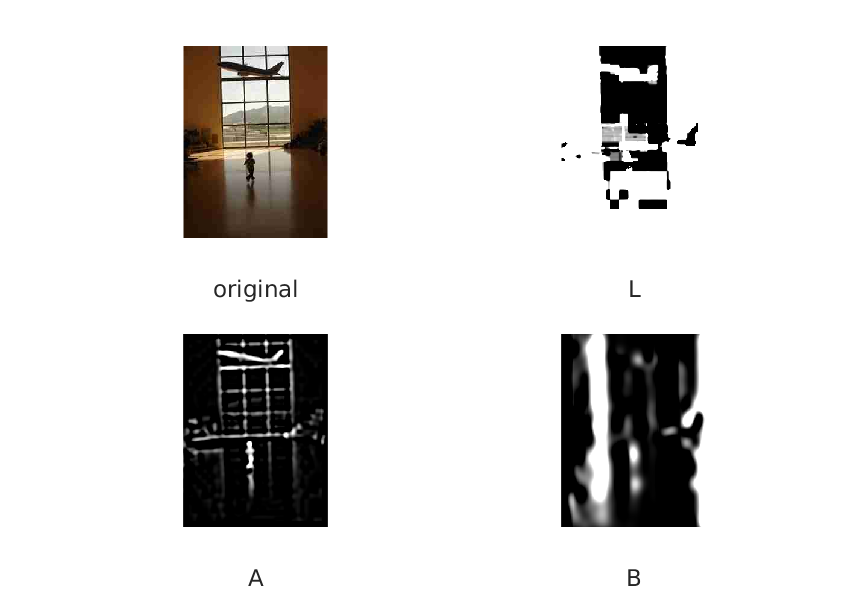
\includegraphics[page=1,width=0.75\textwidth]{q12_extract_filters}
\caption{Filter responses on LAB colored images}    
\label{fig:extract_filter_responses}
\end{figure}   

%%%%%%%%%%%%%%%%%%%%%%%%%%%%%%%%%%%%%%%%%%%%%%%%%%%%%%%%%%%%%%%%%%%%%%%%%%%%%%%%
%%%%%%%%%%%%%%%%%%%%%%%%%%%%%%%%%%%%%%%%%%%%%%%%%%%%%%%%%%%%%%%%%%%%%%%%%%%%%%%%
\newpage
\subsection{Q1.3}

Figure \ref{fig:harris_corners} shows my Harris corner detector applied to three images.

\begin{figure}[H]
\centering
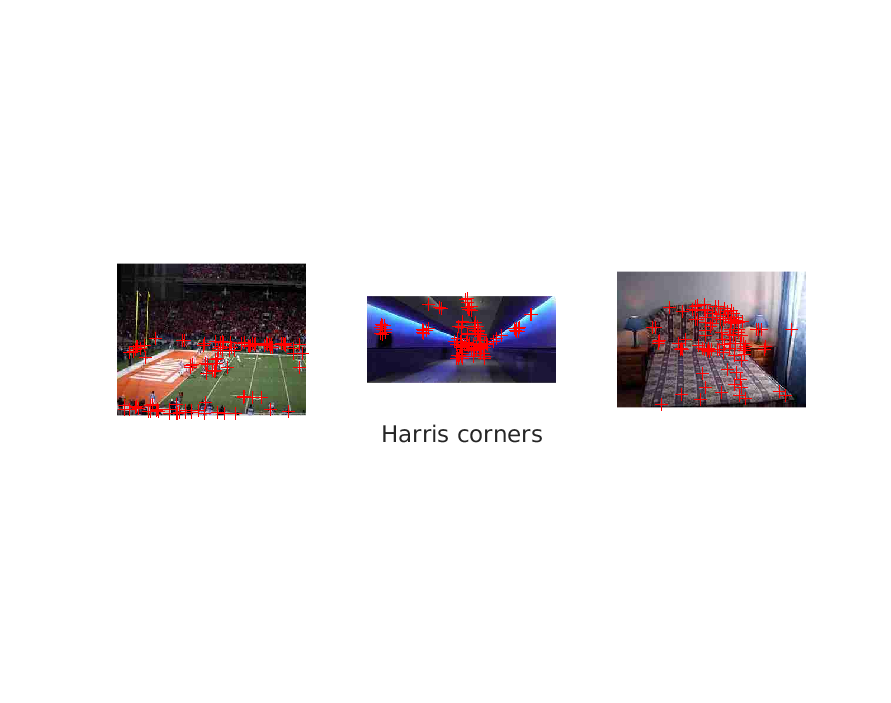
\includegraphics[page=1,width=1\textwidth]{q13_harris}
\caption{Harris corners}    
\label{fig:harris_corners}
\end{figure}   




\end{document}



